\section{Evaluation}
\label{sec:eval}

In this section, we evaluate our parallel congruence closure algorithms on a
number of benchmarks in order to answer the following research questions:

\begin{itemize}
  \item \textbf{RQ1:} Do our two parallel congruence closure algorithms achieve
  a meaningful speedup over a sequential implementation and how does this
  speedup scale with the number of threads?
  \item \textbf{RQ2:} What characterizes the type of benchmark that our parallel
  congruence closure algorithms perform well on?
  \item \textbf{RQ3:} How do our parallel congruence closure algorithms perform
  on real-world benchmarks?
\end{itemize}

We demonstrate the efficacy and limitations of our approach through a wide
selection of benchmarks on various workloads. In \autoref{sec:eval:random}, we
discuss a randomly generated benchmark suite. In \autoref{sec:eval:synthetic},
we discuss a synthetic benchmark suite that allows us to dial up the depth and
width of the benchmark to better understand how these parameters affect the
performance of our algorithms. Finally, in \autoref{sec:eval:circuit}, we
discuss a set of circuit equivalence benchmarks~\cite{clausal-cc}.

All experiments were run on a 96-core Amazon Web Services \texttt{c8i-metal}
instance with Intel(R) Xeon(R) 6975P-C (3.9 GHz) and 384 GB memory. Each core
is 2-way hyperthreaded, giving 192 hyperthreads. The machine runs Ubuntu
26.04 LTS, and the code was compiled using g++ 15.2.0 with -O3.

For each benchmark, we perform 1 warmup run and 5 timed runs, and we report the
geometric mean of the runtime across the 5 timed runs. Throughout this section
we write $T$ for the number of software threads used; in particular, $T{=}1$
denotes the single-threaded configuration of a parallel algorithm.


\subsection{Random Benchmarks}~\label{sec:eval:random}

\begin{figure*}[!tb]
  \centering  \begin{subfigure}[t]{0.48\linewidth}
    \centering
    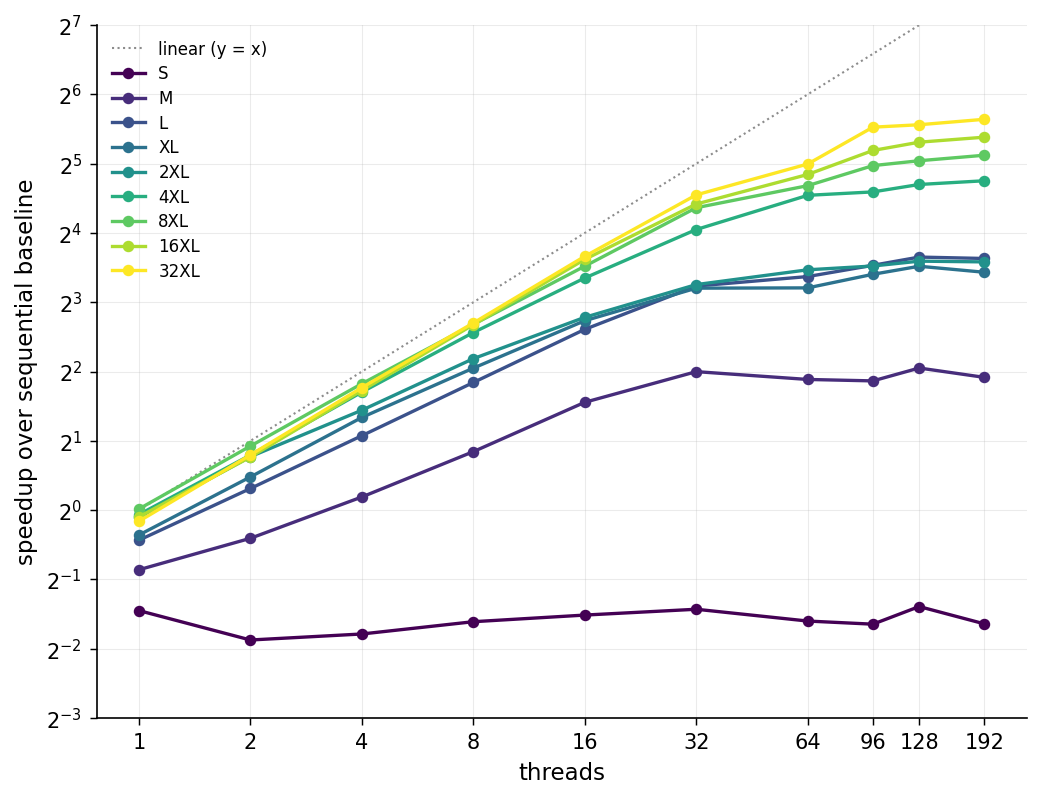
\includegraphics[width=\linewidth]{figs/random_par_parents_speedup_vs_nelson.png}
    \caption{Speedup of \parentalgo compared to sequential baseline.}
    \label{fig:random:parents}
  \end{subfigure}\hfill
  \begin{subfigure}[t]{0.48\linewidth}
    \centering
    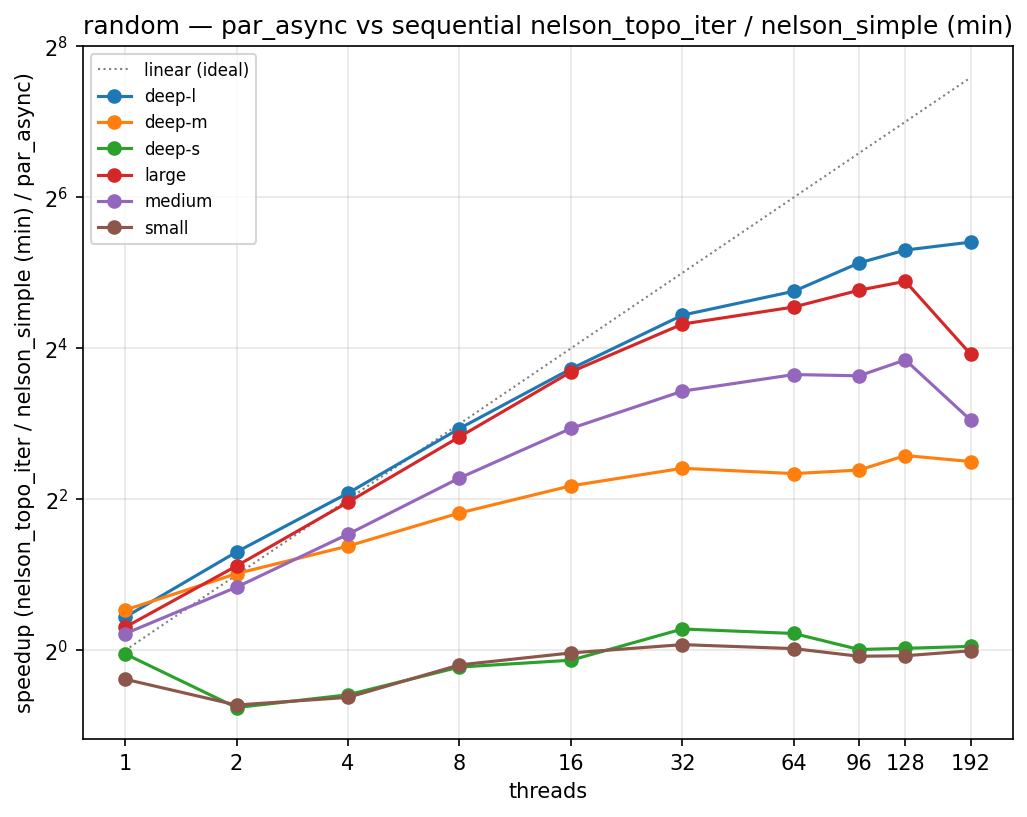
\includegraphics[width=\linewidth]{figs/random_async_speedup_vs_nelson.png}
    \caption{Speedup of \filteralgo compared to sequential baseline.}
    \label{fig:random:filter}
  \end{subfigure}
  \caption{Random benchmarks speedup using \parentalgo and \filteralgo (log-log scale).}
  \label{fig:random}
\end{figure*}


Our first set of benchmarks are randomly generated based on several
parameters. We first define a set of function symbols $F$, which has
$n_{\text{fns}}$ total functions. Then we have a set of terms $\mathcal{T}$ that
contains $n_{\text{leaves}}$ \texttt{x}-leaves and $n_{\text{leaves}}$
\texttt{y}-leaves, plus $n_{\text{compound}}$ compound terms of \emph{depth}
$d$ (i.e.\ with $d$ nested function applications). We initially start with
the equalities $E = \{x_{i_1} = y_{i_1}, \ldots, x_{i_{n_{\text{merges}}}} =
y_{i_{n_{\text{merges}}}}\}$, i.e.\ $n_{\text{merges}}$ random equalities
where each pair contains one \texttt{x}-leaf and one \texttt{y}-leaf.
Essentially, this setup divides the set of leaves into two halves. We
stratify our workloads into different size classes, which are shown in
\autoref{tab:workloads}.


% Our first set of benchmarks is parameterized by several parameters. $l$
% denotes the number of leaves---i.e. the ``variables'' that appear within
% terms. $w$ denotes the \emph{width} of the benchmark: how many equalities are
% initially given before computing their congruence closure. The parameter $n$
% denotes the total number of \emph{nodes}, which are non-leaf terms (e.g.
% function applications). The \emph{depth} $d$ denotes the depth of the terms,
% or how many nested function applications appear in the term. For example, the
% term $f(g(h(x)))$ has depth 2, and the term $x$ (a single variable) has depth
% 0. The parameter $f$ denotes the number of function symbols. Finally, the
% parameter $p$ denotes the number of software threads.




% \as{I think we should only report the deep versions of these benchmarks. I
% update the table to rename things}

\begin{table}[!tb]
  \centering
  \begin{tabular}{l r r r r r}
    \toprule
    workload & $n_{\text{leaves}}$ & $n_{\text{compound}}$ & $n_{\text{merges}}$
    & depth & $n_{\text{fns}}$ \\
    \midrule
    % \texttt{small}   &      1\,000 &     10\,000 &      2\,000 & 1 &  4 \\
    \texttt{small}  &      1\,000 &     10\,000 &      2\,000 & 3 &  4 \\
    % \texttt{medium}  &     10\,000 &    200\,000 &     20\,000 & 1 &  8 \\
    \texttt{medium}  &     10\,000 &    200\,000 &     20\,000 & 3 &  8 \\
    % \texttt{large}   &     50\,000 &  1\,000\,000 &    100\,000 & 1 & 16 \\
    \texttt{large}  &     50\,000 &  1\,000\,000 &    100\,000 & 3 & 16 \\
    \texttt{xl}   &    100\,000 &  2\,000\,000 &    200\,000 & 3 & 16 \\
    \texttt{2xl}  &    200\,000 &  4\,000\,000 &    400\,000 & 3 & 16 \\
    \texttt{4xl}  &    400\,000 &  8\,000\,000 &    800\,000 & 3 & 16 \\
    \texttt{8xl}  &    800\,000 & 16\,000\,000 & 1\,600\,000 & 3 & 16 \\
    \texttt{16xl} &  1\,600\,000 & 32\,000\,000 & 3\,200\,000 & 3 & 16 \\
    \texttt{32xl} &  3\,200\,000 & 64\,000\,000 & 6\,400\,000 & 3 & 16 \\
    \bottomrule
  \end{tabular}
  \caption{Random workload parameters. We have $n_{\text{fns}}$ function
  symbols, each of arity $2$. Each workload has $n_{\text{leaves}}$
  \texttt{x}-leaves plus $n_{\text{leaves}}$ \texttt{y}-leaves at the base,
  $n_{\text{compound}}$ compound terms of depth $d$ built from
  uniformly-chosen function symbols, and $n_{\text{merges}}$ random initial
  equalities, each pairing one \texttt{x}-leaf with one \texttt{y}-leaf.
  % All workloads use a fixed merge-density ratio $n_{\text{merges}} /
  % n_{\text{leaves}} = 2$ and a constant scaling $n_{\text{compound}} /
  % n_{\text{leaves}} = 20$.
  }
  \label{tab:workloads}
\end{table}


% \as{add analysis here}

\autoref{fig:random} shows the speedup of our parallel algorithms over the
sequential baseline. We observe that on workloads with more nodes, our
algorithms achieve close to linear speedup, plateauing between 32 and 64
threads. For instance, on \texttt{32xl}, \filteralgo (resp.\ \parentalgo)
achieves a speedup over sequential of $36.8\times$ ($23.4\times$) on 32
threads, $51.9\times$ ($31.9\times$) on 64 threads, and $76.1\times$
($50.0\times$) on 192 threads.

While both \parentalgo and \filteralgo achieve similar parallelization on
larger workloads, \filteralgo's single-thread runtime is much better than
\parentalgo's. This is because \parentalgo must maintain a parent list for
each term, which is expensive due to the frequent allocations required.
The sequential algorithm also maintains parent lists, but is able to avoid
duplicates.


Note that on sufficiently large workloads we observe \emph{superlinear}
speedups, e.g., \filteralgo on \texttt{32xl} reaches $36.8\times$ on 32
threads. We believe this is because \filteralgo has fewer data structures
to maintain, so on larger workloads the sequential version suffers more
from cache misses and other memory overhead. In particular, maintaining
parent lists in the sequential algorithm (and in \parentalgo) has poor
spatial locality, since the children of a term may be scattered far from
the parent in memory.

% While varying the number of nodes, leads to better speedups, the results for
% varying the depth is more complicated. For instance, while \texttt{deep-s} and
% \texttt{deep-l} achieve greater speedups than their less deep counterparts,
% \texttt{deep-m} achieves a smaller speedup than \texttt{medium}. This is
% likely because the depth of the benchmark affects the number of rounds of
% congruence closure. Our algorithm only parallelizes over the merges within a
% round, but not over the total number of rounds. We evaluate this further in
% \autoref{sec:eval:synthetic}.



\subsection{Synthetic Benchmarks}~\label{sec:eval:synthetic}

\begin{figure*}[!tb]
  \centering
  \begin{subfigure}[t]{0.48\linewidth}
    \centering
    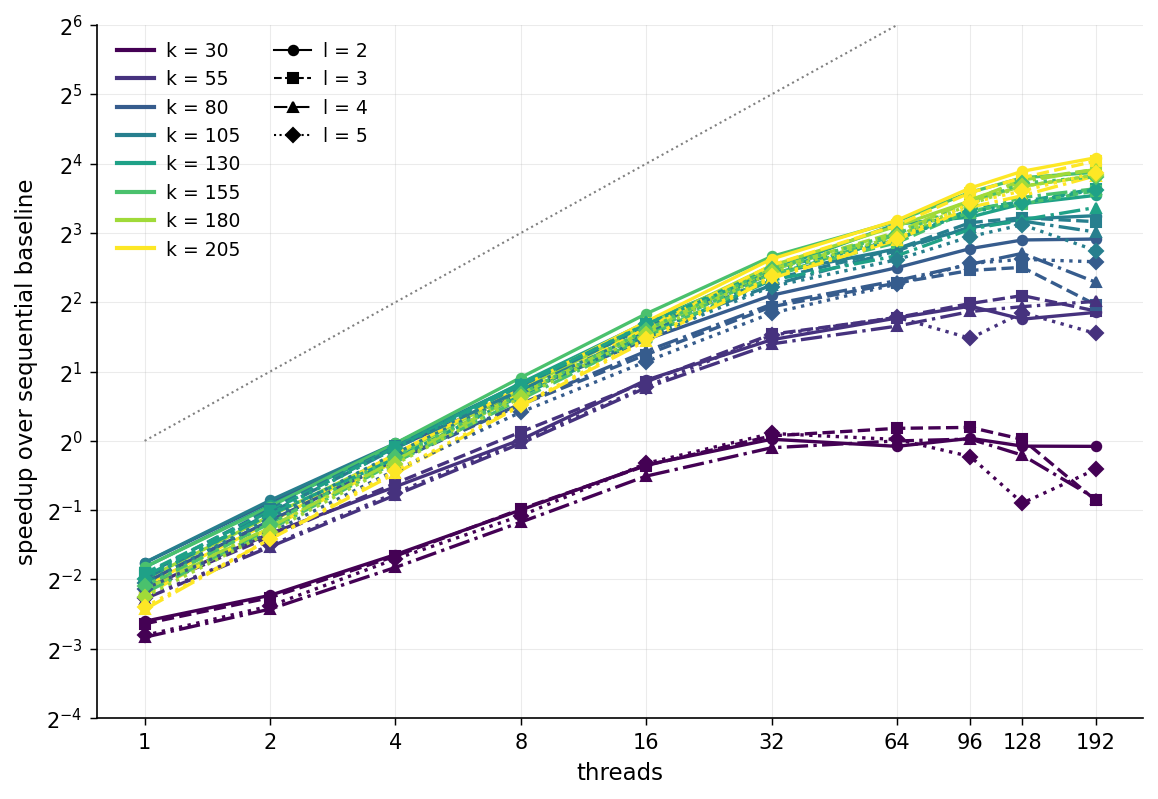
\includegraphics[width=\linewidth]{figs/cube_decomp_par_parents_speedup_vs_nelson.png}
    \caption{Speedup of \parentalgo compared to sequential baseline.}
    \label{fig:synthetic:parents}
  \end{subfigure}\hfill
  \begin{subfigure}[t]{0.48\linewidth}
    \centering
    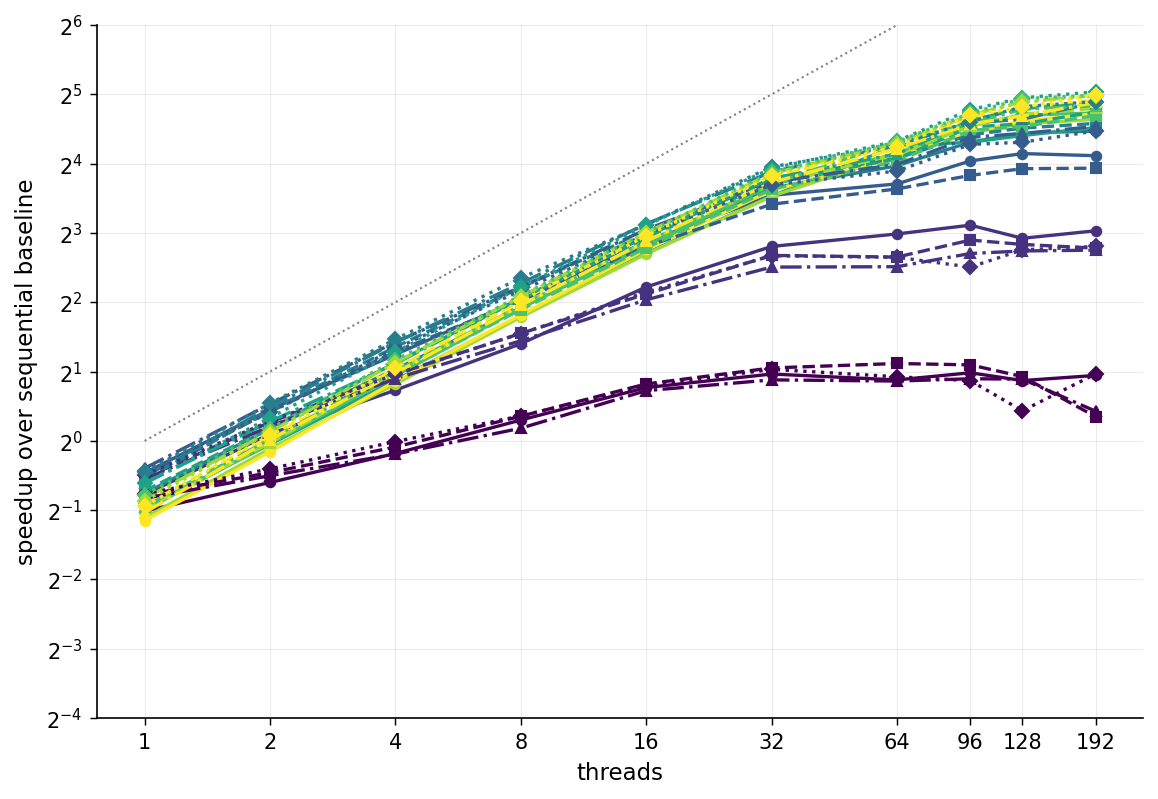
\includegraphics[width=\linewidth]{figs/cube_decomp_async_speedup_vs_nelson.png}
    \caption{Speedup of \filteralgo compared to sequential baseline.}
    \label{fig:synthetic:filter}
  \end{subfigure}\hfill
  \caption{Synthetic benchmarks speedup using \parentalgo and \filteralgo.}
  \label{fig:synthetic}
\end{figure*}

To better understand the relationship between the depth (i.e. number of rounds
of congruence closure) and the width (i.e. number of merges per round) of the
benchmark and the performance of our algorithm, we design a synthetic benchmark
suite that allows us to dial up these parameters.

Our benchmark suite is parameterized by a width $k$ and a $g$-tree fan-in
$l$, and is constructed in three layers:

\begin{itemize}
  \item \textbf{Leaves.} $2k$ leaf constants $a_1, \ldots, a_k$ and $b_1,
        \ldots, b_k$.
  \item \textbf{$f$-layer.} For every triple $(i, j, m) \in \{1, \ldots,
        k\}^3$ we add the terms $f(a_i, a_j, a_m)$ and $f(b_i, b_j, b_m)$,
        contributing $2k^3$ terms in total.
  \item \textbf{$g$-tree.} On each of the $a$- and $b$-sides we build a
        balanced $l$-ary tree of $g$-applications whose leaves are the $k^3$
        $f$-terms on that side. Each internal $g$-node has exactly $l$
        children, and the tree has height $\lceil \log_l(k^3) \rceil$. The
        two sides share no $g$-nodes.
\end{itemize}

The initial unions are $a_i = b_i$ for $i \in \{1, \ldots, k\}$. After
congruence closure has propagated these unions through the $f$-layer there are
$k^3$ congruences of the form $f(a_i, a_j, a_m) \equiv f(b_i, b_j, b_m)$, which
must in turn propagate up the two $g$-trees until the two roots become equal.

The width $k$ controls how many merges occur at the first congruence-closure
round above the leaves: a larger $k$ means a much larger frontier ($k^3$
merges) of mutually-independent $f$-equalities, all of which can be discharged
in parallel. The fan-in $l$ controls the height of the $g$-tree above the
$f$-layer: each level reduces the active frontier by a factor of $l$, so a
larger $l$ produces a shallower closure (fewer rounds) at the cost of wider
fan-in per $g$-node. We sweep $k \in \{30, 55, 80, 105, 130, 155, 180, 205\}$
and $l \in \{2, 3, 4, 5\}$.

\autoref{fig:synthetic} reports the speedup of both algorithms over the
sequential baseline across this sweep.
We see that the width of the benchmark has a much larger impact on the speedup
than the depth. Holding $k$ and thread count $T$ fixed, the parallel
speedup varies by only $\sim$20\% across the four tree depths we measured
(median max/min over $l$ of $1.21\times$ for \filteralgo and $1.20\times$ for
\parentalgo), demonstrating that depth has negligible impact on parallel
performance. This ratio is roughly constant across thread counts, ranging from
$1.15\times$ at $T{=}8$ to $1.31\times$ at $T{=}128$ for \filteralgo, and from
$1.13\times$ at $T{=}4$ to $1.29\times$ at $T{=}192$ for \parentalgo. Holding
$l$ and thread count fixed, on the other hand, varying $k$ produces a much wider
speedup spread (median max/min over $k$ of $5.97\times$ for \filteralgo and
$4.87\times$ for \parentalgo). Unlike the depth ratio, the width ratio grows
sharply with thread count: at $T{=}1$ it is $1.49\times$ for \filteralgo and
$1.78\times$ for \parentalgo, but by $T{=}192$ it reaches $20.2\times$ and
$23.2\times$ respectively.

Similar to the random workloads, our algorithms achieve near-linear speedup
over the sequential version up to a plateau between 32 and 64 threads.
However, the single-core baseline is noticeably worse than the sequential
algorithm: at $k{=}205$, $l{=}2$, \filteralgo at $T{=}1$ is $2.22\times$
slower than the sequential algorithm and \parentalgo at $T{=}1$ is
$4.25\times$ slower. On the same workload, \filteralgo (resp.\ \parentalgo)
achieves a speedup over sequential of $6.79\times$ ($3.30\times$) on 16
threads, $12.3\times$ ($6.16\times$) on 32 threads, $17.0\times$
($9.09\times$) on 64 threads, and $26.4\times$ ($17.0\times$) on 192
threads.



% \autoref{fig:cube:loglog} shows the runtime of our parallel congruence closure
% algorithm on this benchmark suite. We observerve that increasing $k$ and hence
% the width of the benchmark leads to better speedups, while decreasing $d$ and
% hence increasing the depth of the benchmark has minimal impact. The speedups
% are around half as good as a full linear speedup and start to plateau around
% $64$ cores. For instrance, for $k=155$ and $d=5$, we achieve speedups of
% $7.47\times$ on 16 cores, $13.89\times$ on 32 cores, $21.4\times$ on 64 cores,
% and $29.7\times$ on 128 cores.

% Overall, we can conclude that our algorithm performs well on benchmarks with a
% large number of merges per round, and is not significantly affected by the
% total number of rounds of congruence closure.




\subsection{Circuit Equivalence Benchmarks}~\label{sec:eval:circuit}

% In this section, we evaluate on a set of benchmarks checking the equivalence
% of two circuits. The canonical way to check circuit equivalence is using a
% miter, a construction where given two circuits $C_1$ and $C_2$ (with the same
% number of inputs and outputs), we construct a new circuit $M$ that (1) for
% each output of $C_1$ and $C_2$, takes their XOR and (2) ORs all the XOR
% results together. Then if $M$ is unsatisfiable, i.e. the output on any set of
% inputs is always $0$, then $C_1$ and $C_2$ are equivalent.


% Typically, the miter is converted into conjunctive normal form (CNF) and given
% to a SAT solver. However, these formulas can be very large and difficult to
% solve. Biere et al.~\cite{clausal-cc} showed that the two sides of a miter
% often share equivalent sub-circuits whose equivalence can be discovered
% structurally, allowing the formula to be simplified significantly using
% congruence closure.

% % often different circuits have redundant subcircuits and % thus these
% formulas can be simplified significantly using congruence closure.

% Biere et al. evaluated their clausal congruence closure algorithm on two
% benchmark sets: five circuit pairs that were curated to be hard for monolithic
% CNF-level SAT sweeping~\cite{iwls} and a set of benchmarks comparing an
% original circuit against either (1) an optimized or (2) an isomorphic version
% of itself~\cite{hwmcc}. They implemented their congruence closure algorithm as
% a preprocessing pass in the SAT solver Kissat~\cite{kissat} and showed that it
% significantly reduced the time taken to solve these benchmarks. For our
% evaluation, we modify Kissat to expel the congruence closure problem before .
% We modify the benchmarks slightly so that instead of treating negation as a
% specific boolean connective, we treat it as a function symbol.

These benchmarks come from the clausal congruence closure work of Biere
et al.~\cite{clausal-cc}, which (as discussed in
\autoref{sec:bg:motivating}) uses congruence closure over recovered gates to simplify
miters before SAT solving. They implemented their algorithm as a
preprocessing pass in Kissat~\cite{kissat} and evaluated on two benchmark
sets: 10 hand-curated miters from the IWLS'22 paper~\cite{iwls},
considered hard for monolithic CNF-level SAT sweeping, and a derivative
of the 2012 Hardware Model Checking Competition~\cite{hwmcc} that
compares each And-Inverter Graph against an optimized variant.

For our evaluation we use the same circuit sources, but rather than
running congruence closure as a preprocessing pass within Kissat we
extract its intermediate gate set and run our parallel congruence closure
implementations on it directly. Concretely, we instrument Kissat's gate
extractor to dump every candidate gate (AND/XOR/ITE) and run our
congruence closure implementations on these gates. From the HWMCC'12 set
we pick the twelve hardest instances by sequential congruence closure
time.

\begin{figure*}[!tb]
  \centering
  
  \begin{subfigure}[t]{0.48\linewidth}
    \centering
    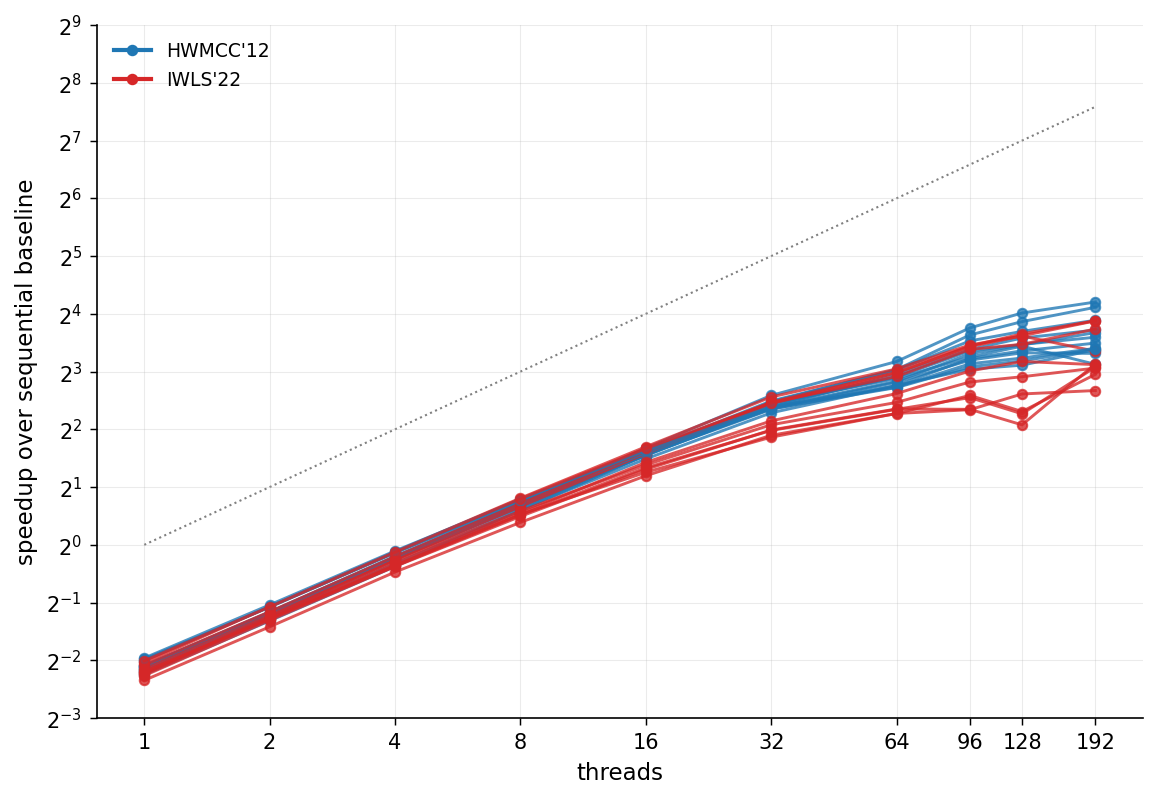
\includegraphics[width=\linewidth]{figs/gates_par_parents_speedup.png}
    \caption{Speedup of \parentalgo compared to sequential baseline.}
    \label{fig:circuit:parents}
  \end{subfigure}\hfill
  \begin{subfigure}[t]{0.48\linewidth}
    \centering
    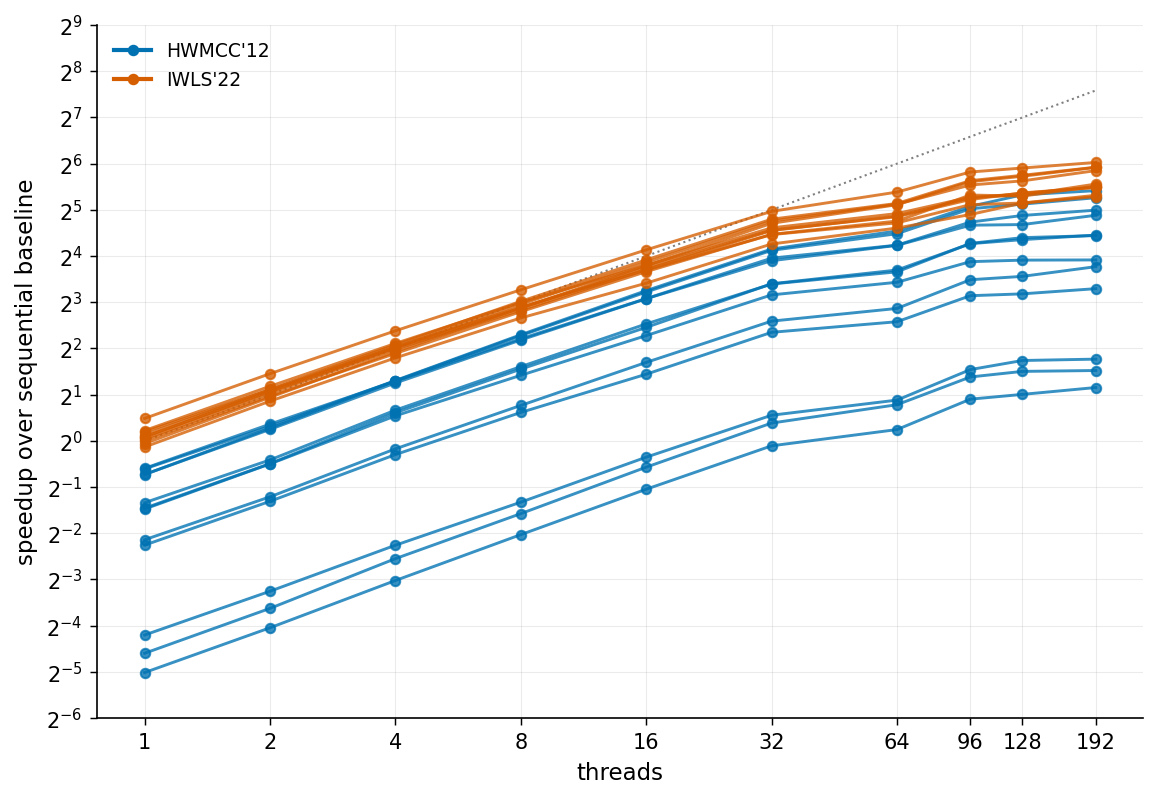
\includegraphics[width=\linewidth]{figs/gates_async_speedup.png}
    \caption{Speedup of \filteralgo compared to sequential baseline.}
    \label{fig:circuit:filter}
  \end{subfigure}
  \caption{Speedup of \parentalgo and \filteralgo on circuit equivalence benchmarks.}
  \label{fig:circuit}
\end{figure*}

% \as{add analysis and make below more clear (comment + add explanation of the figures)}

% We do not compare to Kissat's internal congruence closure implementation as our
% sequential implementation was much faster compare to the numbers reported in the
% paper~\cite{clausal-cc}.

\autoref{fig:circuit} reports the speedup of both algorithms over the
sequential baseline on these benchmarks as the thread count $T$ is varied.
On the circuit-equivalence benchmarks, \filteralgo and \parentalgo achieve
near-linear speedup up to a plateau between 32 and 64 threads on most
workloads. However, unlike on the random and cube benchmarks, the single-thread
runtime of \filteralgo varies dramatically across files. On the 22 files we
measured, its runtime at $T{=}1$ ranges from $0.71\times$ the sequential runtime
on \texttt{h5m-n04-ands.gates}---the one file where \filteralgo outperforms
sequential even on a single thread---up to $32.3\times$ the sequential runtime on
\texttt{6s104-xits-opt.gates}. \parentalgo, by contrast, is consistently
$\sim$$4\times$ slower than sequential at $T{=}1$ regardless of file.

\begin{figure}[H]
  \centering
  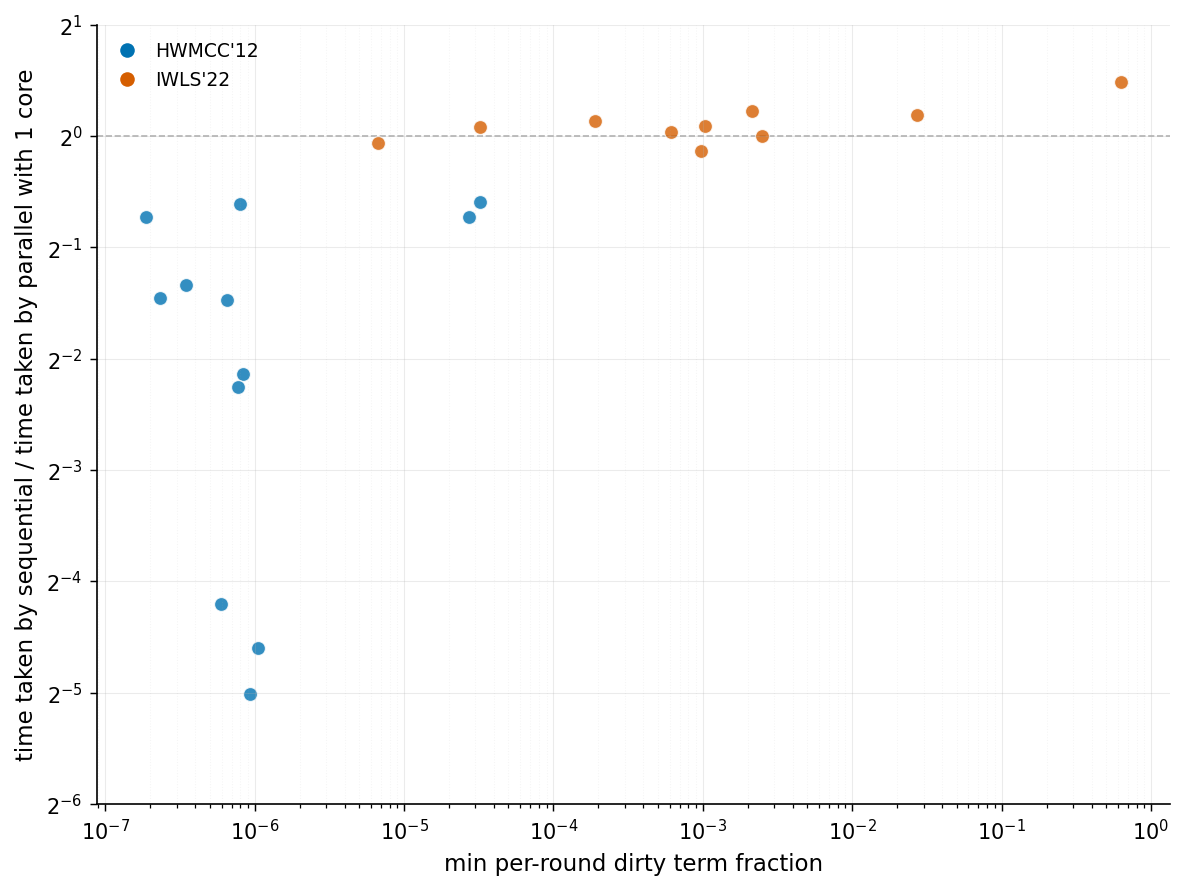
\includegraphics[width=\linewidth]{figs/gates_speedup_vs_min_dirty_fraction.png}
  \caption{Slowdown of \filteralgo compared to sequential baseline vs.\ the smallest fraction of dirty terms across rounds.}
  \label{fig:gates_vs_min_dirty_fraction}
\end{figure}

\autoref{fig:gates_vs_min_dirty_fraction} explains this spread by plotting
the speedup of \filteralgo against the \emph{minimum per-round dirty term
fraction}: for each round $r$ of the algorithm we record
$\mathrm{dirty}[r]/\mathrm{live}[r]$, where $\mathrm{dirty}[r]$ is the number of
terms the round marks as needing re-canonicalization and $\mathrm{live}[r]$ is
the number of equivalence classes still alive after the preceding round's
unions; we then take the minimum over all rounds the closure executes. A small
minimum is bad for \filteralgo because every round, regardless of how few terms
are actually dirty, pays the full $O(\mathrm{live})$ cost of scanning all live
terms to filter out the dirty ones --- so a workload with even one near-empty
round wastes work proportional to all live terms for very few useful unions.
% The figure shows a strong positive correlation (Spearman $\rho{\approx}{+}0.79$)
% between the minimum dirty fraction and the per-file speedup, and exactly the
% files with very low minimum fractions — \texttt{6s104-ands/xits-opt},
% \texttt{6s163-xits-opt}, and a couple of others — are the ones where \filteralgo
% is many times slower than sequential at $T{=}1$ and where \parentalgo (which has
% no such filter) is faster at every thread count.

%  To address the concern that
% good speedups are an artifact of small workloads, we highlight
% \texttt{6s125-ands-opt.gates}, the largest closure in the suite at $5.5$~seconds
% sequentially: on this workload \filteralgo (and respectively \parentalgo)
% achieves a speedup over sequential of $9.33\times$ ($2.94\times$) on 16 threads,
% $17.4\times$ ($5.56\times$) on 32 threads, $22.4\times$ ($8.20\times$) on 64
% threads, and $38.4\times$ ($17.3\times$) on 192 threads.






% \subsection{Equality Saturation Benchmarks}

% To get equality saturation benchmarks, we ran egglog~\cite{egglog} on the
% egg-cc project~\cite{eggcc}—an experimental optimizing compiler for the
% LLVM-like IR Bril. We ran egglog on a number of Bril programs for \as{todo}
% seconds and logged all of the unions egglog generated during this time. We
% then extracted these unions into an SMT-LIB file and evaluated our parallel
% congruence closure algorithms on these benchmarks.

% \subsection{SMT Benchmarks}

% To get SMT benchmarks, we took benchmarks from the QF-UF logic in the annual
% 2025 SMT competition~\cite{smtcomp2025}. In this category, we picked the
% benchmarks from \asm{fill in} as the other benchmarks were either very simple
% or required more complicated boolean reasoning.

% These benchmarks include boolean connectives, so to get pure congruence
% closure constraints, we ran each of the bencmarks through the Sundance-SMT
% solver ~\cite{sundance}, every time Sundance-SMT found a conflict in its
% congruence closure solver, we extracted the set of equalities into an SMT-LIB
% file.





